\documentclass{article}
\usepackage[T1]{fontenc}
\usepackage[utf8]{inputenc}
\usepackage[english]{babel}
\usepackage{amssymb,amsmath,amsthm,mathtools} 
\usepackage{tikz-cd,wrapfig}
\usepackage{tcolorbox}
\usepackage{graphicx}
\usepackage{wrapfig}
\usepackage{pdfpages}
\usepackage{enumitem}
\usepackage{pdfsync}
\usepackage{amstext} % for \text macro
\usepackage{array}   % for \newcolumntype macro
% \newcolumntype{C}{>{$}c<{$}} % math-mode version of "C" column type
%Personal package
\usepackage{listings}
\usepackage{lstlang0}
\usepackage{bm}
\usepackage{csquotes}


%Commands
\newcommand{\DD}{\mathcal{D}}
\newcommand{\ZZ}{\mathbb{Z}}
\newcommand{\PP}{\mathbb{P}}
\DeclareMathOperator{\sgn}{sgn}
\newcommand{\WW}{\mathcal{W}}
\newcommand{\FT}{\mathcal{F}}
\newcommand{\F}{\mathbb{F}}
\newcommand{\BB}{\mathcal{B}}
\DeclareMathOperator*{\eqb}{=}
\DeclareMathOperator{\ifff}{\iff}


% Theorem definitons 
\theoremstyle{plain}
\newtheorem{teo}{Theorem}[section]
\newtheorem{lem}[teo]{Lemma}
\newtheorem{prop}[teo]{Proposition}
\newtheorem{cor}[teo]{Corollary}
\newtheorem*{form}{Formula}

\theoremstyle{remark}
\newtheorem{rem}{Remark}
\newtheorem{rems}[rem]{Remarks}
\newtheorem{idea}[rem]{Idea}


\theoremstyle{definition}
\newtheorem{deff}[teo]{Definiton}
\newtheorem{algo}[teo]{Algorithm}
\newtheorem{prob}[teo]{Problem}
\newtheorem*{nota}{Notation}

%Bibliography
\usepackage[backend=biber, style=alphabetic, maxnames = 8, giveninits=true,isbn=false,eprint=false]{biblatex}
%other_styles:numeric_authortitle
\addbibresource{biblio.bib}


\usepackage{hyperref}



\title{Report for the MAGMA project}
\author{Giacomo Borin}

\begin{document}

\maketitle

\begin{abstract}
	The report contain the implementation of 5 algorithms:
	\begin{itemize}
		\item ECDSA, a digital signature scheme based on algebraic curves.
		\item Pohlig Hellman alorithm for solving discrete logarithm problem for Algebraic curves. Particularly efficient when the base point has order with only small primes in the factorization
		\item Index Calculus algorithm for solving discrete logarithm problem for in finite fields of prime order using linear algebra and B-smooth sieving.
		\item Solovay-Strassen primality test, based on the evaluation of the Jacobi Symbol.
		\item Lehman factorization algorithm, based on a modification of the Fermat factorization algorithm.
	\end{itemize}


\end{abstract}

\subsection*{General considerations}

In general functions already implemented in MAGMA are significantly faster than ours, so when possible we have used them. 


\section{ECDSA}

ECDSA is a Digital Singature Algorithm based on elliptic curves proposed by \cite{ECDSA} based on the difficulty of the discrete logarithm on them. 

The public setup of the scheme is composed by the finite field $\F_q$, an elliptic curve $E = E(\F_q)$ and a base point $G$ with order a large prime $r$. Then Alice can generate a private key $d\in \{2,..,r-1\}$ and publish the public key $d\cdot G$. The message is an integer $m$ (usually it is the hash of the message) and to sign it Alice has to perform:
\begin{enumerate}
	\item Choose a random $k$ with $1 \leq k < r$.
	\item Evaluate $R = k \cdot G$.
	\item Evaluare $ s = (m + d\cdot R_x) k^{-1} \mod r$, where $R = (R_x : R_y : 1)$.
\end{enumerate}
The signature of $m$ is then $(R,s)$.

To verify it Bob has to:
\begin{enumerate}
	\item Compute $u_1 = s^{-1} m \mod r$ and $u_2 = s^{-1} R_x  \mod r$.
	\item Evaluate $V = u_1 \cdot G + u_2 \cdot Q$. 
	\item The signature is valid if $V = R$.
\end{enumerate}

\begin{teo}
	Alice is generating a valid signature for each choices of the parameters
\end{teo}
\begin{proof}
	We simply do the computation recalling that the calculations on the coefficents are done modulo the order $r$:
	\begin{multline*}
		V = u_1 \cdot G + u_2 \cdot Q = s^{-1} \cdot m \cdot G + s^{-1} \cdot R_x \cdot (d \cdot G) = \\
		= s^{-1} (m + d\cdot R_x) \cdot G = k\cdot (m + d\cdot R_x)^{-1} (m + d\cdot R_x) \cdot G = \\
		= k \cdot G = R
	\end{multline*}
\end{proof}


\subsection{Implementation choiches}

We have implemented the algorithm from~\cite[Section 6.6]{washington}.

I've personally implemented all the code and a good part of the test vectors (it didn't took a lot of time), while Dario helped with debugging. The code is the plain transposition of the previous instructions in MAGMA, using the \texttt{EllipticCurve} operations, so there isn't much to say. I will reacall only some small observations.

We can see that it would be faster to use a small $k$ (for example $k = 4$ as Sony), since it simplifies a lot the evaluation of $kG$ (in fact $k=4$ would require only two doublings) but it would be very bad for security. 
However I have tried to use again the idea, considering $k \in [-\frac{r}{2}, \frac{r}{2}]$, so that the modulus is sligtly smaller and we save some doublings. To do this I have also defined the function \texttt{mmod(a,m)} that returns an integer in $[-\frac{r}{2}, \frac{r}{2}]$ equalt to $a$ modulo $m$. This idea saves only a small time ($0.1$ seconds)\footnote{Some evaluation can be seen in the \href{https://github.com/giacomoborin/project2_MAGMA/pull/36}{associated pull request}}.

Another observation is that we have used \texttt{Modinv} to find the inverses modulo $r$ and in the verification algorithm we evaluate $s^{-1}$ only one time. Sadly we had to use two casts, since the coordinates of the point \texttt{R} and in the finite field, but we need type \texttt{Integers()} to perform the moltiplications. 

%\begin{lstlisting}[language = magma]
%> load "ECDSA.mag"; // k random
%Loading "ECDSA.mag"
%> load "Test_ECDSA.mag";
%Loading "Test_ECDSA.mag"
%Time: 6.130
%> load "ECDSA.mag"; // k = 4    
%Loading "ECDSA.mag"
%> load "Test_ECDSA.mag";
%Loading "Test_ECDSA.mag"
%Time: 4.230
%\end{lstlisting}


Another simple idea is to evaluate only once the inverse of $s$, it saves only $0.1$ seconds, but it is still worth it (you can see more on \href{https://github.com/giacomoborin/project2_MAGMA/issues/13}{the relative issue on github}).

\section{Pohlig-Hellman}

The Pohlig-Hellman method is an algorithm for the evaluation of the discrete logarithm %with base element of finite order
, i.e. given $P$ and $Q$ in a group $G$ such that $P$ has finite order $N$ and exists $k\in \{0,...,N-1\}$ such that $kP = Q$ the algorithm finds $k$. 

\begin{nota}
	I will use additive notation for the group operation with neutral element $O$ since we are requested to implement this algorithm for solving discrete logarithm for Elliptic Curves. 
\end{nota}

\begin{idea} \label{idea:ecdlp}
	Consider the factorization:
\begin{equation*}
	N = \prod_{i=1}^r p_i^{e_i}.
\end{equation*}
	Solve now the discrete logarithm modulo $p_i^{e_i}$ for all $i = 1,...,r$ and use these values to evaluate $k$ using the Chinese Reminder Theorem. 
\end{idea}

Let's see a first naive version of the strategy\footnote{I know that this is indeed very similiar to a real code, but for me it is easier to understand} for finding $k \,\text{mod}\, p^e$:

\begin{algo}\label{algo:ecdlp_naive}

	\begin{enumerate}
		\item \label{enum:store} Compute $T = \{ (j,j\left(\frac{N}{p}P\right)) \,|\, j = 0,...,q-1 \}$.
		\item Assign $i := 0$, $Q_0 := Q$
		\item \label{enum:while} find $(j,R)\in T$ such that $R = \frac{N}{p^{i+1}}Q_i$ and assign $k_i := j$
		\item Increment $i := i + 1$, then:
		\item \label{enum:if} If $i < e$ assign $Q_i := Q_{i-1} - k_{i-1} p^{i-1}P$ and return to step \ref{enum:while}
		\item Then we have $k \equiv k_0 + k_1p + ... + k_{e-1}p^{e-1} \mod q^e$ \label{enum:final_dlp}.
	\end{enumerate}

\end{algo}


Obviously the procedure terminates, but we still need to prove that the step \ref{enum:final_dlp} is correct.

\begin{prop}
	\label{prop:corr_dlp}
	Consider $k$ written in base $p$ as $k = \hat{k}_0 + \hat{k}_1p + \hat{k}_2p^2 + ...$, then we have that:

	for each $i \in \{0,...,e-1\}$ at the step \ref{enum:while} hold that 
	$\hat{k}_i = k_i$ and $Q_i = (\hat{k}_ip^i + \hat{k}_{i+1}p^{i+1} + ... )P$
\end{prop}

\begin{proof}
	We will prove this by induction on $i \in \{ 0 ,..., e-1\}$.

	\textbf{Base case}: $i=0$. Trivially we have that $Q_0 = Q = kP = (\hat{k}_0 + \hat{k}_1p + \hat{k}_2p^2 + ...)P$. Observe now that:
	\begin{equation}
		\label{eq:prop:base}
		\frac{N}{p^{0+1}}Q_0 = \frac{N}{p}\hat{k}_0 P + N(\hat{k}_1 + \hat{k}_2p + ...)P \eqb^* \frac{N}{p}k_0 P + O = \hat{k}_0 \frac{N}{p} P
	\end{equation}
	where in $*$ we have used that $NP = O$. Observe that $p$ divides $N$. Since $j$ from step \ref{enum:while} is in $\{0,...,p-1\}$ we have $\hat{k}_0 = j = k_0$.

	\textbf{Induction step}: prove the result for $i \in \{1,...,e-1\}$ assuming that it holds for $i-1$. 

	By the step \ref{enum:if} we have that:
	\begin{multline*}
		Q_i := Q_{i-1} - k_{i-1} p^{i-1}P = (\text{induction on }i-1\text{ for } k_{i-1} \text{ and } Q_{i-1}) \\
		= (\hat{k}_{i-1}p^{i-1} + \hat{k}_{i}p^{i} + ... )P - \hat{k}_{i-1} p^{i-1}P = (\hat{k}_ip^i + \hat{k}_{i+1}p^{i+1} + ... )P.
	\end{multline*}
	So we can evaluate $R$ :
	\begin{multline*}
		\frac{N}{p^{i+1}}Q_i = \frac{N}{p^{i+1}}(\hat{k}_ip^i + \hat{k}_{i+1}p^{i+1} + ... )P = \\
		= \hat{k}_i \frac{N}{p} P + N(\hat{k}_{i+1} + \hat{k}_{i+1}p + ...)P= \hat{k}_i \frac{N}{p} P + O = \hat{k}_i \frac{N}{p} P 
	\end{multline*}
	So in the same way $\hat{k}_i = j = k_i$. Observe that these are the same calculation of the base case and also we have that $p^{i+1}$ divides $N$ since $i<e$. 
\end{proof}

Trivially it follows that:

\begin{cor}
	The result in step \ref{enum:final_dlp} is correct.
\end{cor}

So to find the discrete logarithm we only have to repeat the previous steps for each $p_i^{e_i}$. We can then solve the system 
\[
	k \mod p_i^{e_i} \quad \text{ for } i=1,...,r
\]
using the Chinese Reminder Theorem and get the desired $k \in \{0,...,N-1\}$. 

The strenght of this algorithm is that we are performing the discrete logarithm by linear search $\sum e_i$ times in sets of cardinality $p_i$ (having then a complexity of $O(e_j p_j)$ where $p_j$ is the greatest prime factor) instead of one time for all the $N$ values in $\left< P \right>$. So obviously if the factors of $N$ are small we obtain a result much better than $O(\sqrt{N})$ of other general algorithms (like Shanks or Pollard-Rho). 

For the description (and implementation) of the algorithm I have used \linebreak
\cite[Section 5.2.3]{washington} and \cite[Section 7.2.3]{stinson} (written in multiplicative notation and with a more costructive description). 

\subsection{Implementation}

For now on I will use the same notation used in the code of\\ \texttt{ECDLP}\verb|_|\texttt{PohligHellman(q, E, P, r, Q)}.

Let's start with considering what we have \textbf{not} implemented, i.e. the functions already contatined in MAGMA that we have decided to use since they are more efficient:
\begin{itemize}
	\item \verb|Factorization|, necessary to factor the order of the point \verb|r|
	\item \verb|CRT|, that at the end evaluate the solution of the system modulo \verb|r| of congruences resulting after the for loop.
	\item \verb|IsPrimitive|, I will explain later why we need it.
	\item The \verb|EllipticCurve| \href{http://magma.maths.usyd.edu.au/magma/handbook/elliptic_curves}{structure} and all its functions (in particular the sum and the doubling). 
\end{itemize}

The first working implementation (\href{https://github.com/giacomoborin/project2_MAGMA/blob/2416fa58ca58ef91075fc4a52427d68a5fa182c1/ECDLP.mag}{2416fa5}) of the code followed step by step the Algorithm \ref{algo:ecdlp_naive}. It was very slow because of two principal reasons:
\begin{enumerate}
	\item \label{enum:append} Extensive use of the command \verb|Append|, slow since memory allocation for sequences is expensive, particularly in MAGMA.
	\item \label{enum:map} The use of the command \texttt{map<|>}, similiar to the dictionary in Python, but sadly not efficient in MAGMA. 
\end{enumerate}
The second command was used to perform the steps \ref{enum:store} and \ref{enum:while} of the procedure, that we have individuated as the most time consuming parts of the method:

\begin{prob}[Evaluation]
	Evaluate and store all the values $\{ (j,j\left(\frac{N}{p}P\right)) \,|\, j = 0,...,q-1 \}$ (step \ref{enum:store}). In the code $\frac{N}{p}P$ is \verb|coeffP|. 
\end{prob}

\begin{prop}[Search]
	Search into the evaluated points and return the corresponding index (step \ref{enum:while})
\end{prop}

To solve these problems I have observed that we can consider two different cases: $e=1$ and $e>1$ (where $e$ is the exponent of the prime in the factorization).

\subsection{Case e=1}
Here we can solve the two problems togheter perferming in parallel the evaluation of \verb|j*coeffP| while checking if it is equal to \verb|Qs|. In this way we the memory allocation is negligible and we will need on average \verb|prime|$/2$ operations. 

Let's look more in details to the implementation choices in this case. Obviously we start evaluating \texttt{Qs} (corresponding to $\frac{N}{r}Q$). If it is the infinity point we return directly \verb|k|$=k_0 = 0$ otherwhise we distinguish two other cases. 

In the second one we do the simple evaluation starting from $k = 1$ and $\verb|Point| = \verb|coeffP|$, then increment $k$ by $1$ and \verb|Point| by \verb|coeffP| until we find \verb|Point eq Qs|.

In the first we look if $2$ is primitive in $\mathbb{Z}_p$, in this way to get all the multiples of \verb|coeffP| we can evaluate instead $2^j\verb|coeffP|$ for $j = 0, ..., p-2$. 

So insted of incrementing $k$ we multiply it by $2 \mod p$ and we double \verb|Point|, that is sligtly faster with respect to adding points. (commit \href{https://github.com/giacomoborin/project2_MAGMA/commit/d2d2692170bebfa2b465307761de5c7ee52121bf}{d2d2692})

\subsection{Case e>1}

In this case we go straight with the computation and the storing of points. The only two improvements added where the pre-initialization of the array \verb|T| to reduce new memory allocation and the use of the function \verb|Position| to find the index.

Observe that also \verb|K| and \verb|Qs| where pre-initilized with buffer values. 

\begin{rem} %TODO
	Doing log insted of the search good, but forbidden
\end{rem}


\section{Index Calculus}

The Index Calculus is a method based on linear algebra to solve the discrete logarithm problem in the finite prime fields, i.e. given a generator $g$ and an element $h$ in $ \F_p$ find $x \in \ZZ$ such that $g^x = h$. 

The idea is to fix a factor base $\mathcal{B}$ of primes and find linear relations of $\log_g(b)$ for every $b \in \mathcal{B}$. To do this we compute $\{0,...,p-1\} \ni g_i \equiv g^i \mod p$ for some random integers $i$, if $g_i$ is $\mathcal{B}$-smooth we have that it factors as 
\[
g_i = \prod_{b \in \BB}b^{e_b} \equiv \prod_{b \in \BB} g^{\log_g(b) e_b} \mod p
\]
, thus looking at the exponents we have that:
\begin{equation}
	\label{eq:logp_eq}
	i \equiv \sum_{b \in \BB} e_b \log_g(b) \mod p-1 . 
\end{equation}
So picking random $i$ we can generate enough linear equation \ref{eq:logp_eq} and pick one of the solutions and assume it to contain the logarithms of the primes.

\begin{rems} \label{rem:num_eq}
	Surely the vector with the logarithms is a solution, so if we have an overdetermined system (i.e. with more than $\#\BB$ equations) is possible for it to be the unique solution. Thus a possible way to retrieve it is to consider $\#\BB +1$ equations. We will see later in the implementation that we have done something different, both for correctness and efficiency reason. 

	Also we have that $p-1$ is not a prime, but we need a field to perform correctly Gauss Elimination. We can work out this by doing linear algebra on $\ZZ_q$ for all the prime factors $q$ of $p-1$ and combine them with the Chinese Reminder Theorem. We don't have problems with the powers of the factors since from the specifications we got that $p$ is a safeprime, i.e. $p-1 = 2q$ with $q$ prime. 
\end{rems}

When we have the logarithms of the base we can start to compute $h\cdot g^{-k} \mod p$ for random integers $k$, until we get a $\BB$-smooth number, such that:
\begin{equation*}
	h\cdot g^{-k} \equiv \prod_{b \in \BB} b^{l_b} \mod p
\end{equation*}
At this point we get that:
\begin{equation}
	\label{eq:dlog_final1}
	\log_g(h) \equiv \sum_{b \in \BB} l_b \cdot \log_g(b) \mod p-1
\end{equation}

This algorithms works with some attention to the remark during the implementation, but I have found a better version of it in these \href{https://math.mit.edu/classes/18.783/2021/LectureNotes10.pdf}{lecture notes}. 
Here in fact the two steps are united togheter: instead of considering $g^i$ to find the equations for the linear system we consider directly $h\cdot g^{-k} \mod p$, if it is $\BB$-smooth from the factorization we get an equation:

\begin{equation}
	\label{eq:dlog_final2}
	k \equiv \log_g(h) - \sum_{b \in \BB} e_b \cdot \log_g(b) \mod p-1
\end{equation}

So if we consider a system of linear equations of the form \ref{eq:dlog_final2} surely it contains as solution a vector with first component equal to $\log_g(h)$. I have verified that this method is computationally more efficient, and I thinks that there are two reasons:
\begin{itemize}
	\item It is more compact, with a single linear system we can directly get a candidate solution. 
	\item We need only to look for the first component of the solution\footnote{technically in the implementation it will be the last, but it doesn't matter}, so even if all the others are wrong, but the solution space intersect the line $\left< (1,0,...,0)\right>$ in a single point we are sure that it is the solution. 
\end{itemize}

\begin{rem}
	A question that I asked myself was: \textit{but what about the other solutions? Can I try to use them?} The answer is no, in fact the intersection of a line with an affine subspace is an affine subspace that can have only dimension $0$ (so it's a single point) or dimension $1$, thus it is the line itself (of cardinality $p-1$). So looking to the other solutions (if not unique) is equivalent to use brute force.
\end{rem}

Reference for \textit{index calculus} can be found in \cite[Section 7.2.4]{stinson}.

\subsection{Implementation}

Dario had done the first implementation, using the first version, but there were some problems and some possible improvements. The principal one was that not every solution of the linear system gives the discrete logarithm. I had tried to solve in two ways:
\begin{itemize}
	\item Removing columns with all zeros. In fact in this case we don't have condition on the corresponding coordinate, so all the possible values are accettable. The idea at this point is to consider a factor base that contains only the primes with non zero columns modulo $q$ and $2$. A possible way to implement this can be seen in the commit \href{https://github.com/giacomoborin/project2_MAGMA/pull/30/commits/4b0b67d0dcbe51f01058c64a06a1c39fdb5cf56e}{4b0b67d}.
	\item Since the previous solution isn't enough I have inserted a check to see if the solution is effectively the discrete logarithm, if not the function generate more equations and tries to find a new solution.  
\end{itemize}

When I have implemented the second version the filtering on the columns was no longer necessary, but still we need to use an iterative strategy. 

Let's look at the final algorithm. It starts with the creation of the factor base, in particular it is done by choosing a bound \texttt{TopB} and using $\BB $$= \{ p \,|\, p \text{ prime and } p \leq \verb|TopB|\}$ (evaluated with the MAGMA function \texttt{PrimesUpTo} ). You can read more on this in the section \ref{sssec:fact_base}. 

Then we can initialize some bounds (explained in section \ref{sssec:bounds}) and two counter, \texttt{rows} and \texttt{newrows}, a random \texttt{exponent} and start the algorithm. Using \\ \texttt{Factorization} we factor $h\cdot g^{-k} \mod p$ and memorize its decomposition. Then se can see if it is $\BB$-smooth directly verifying the containment of the primes in the decomposition into \texttt{B}.

\begin{rem}
	Mathematically, to see if a number $n$ is $\mathcal{B}$-smooth and get its factorization it should be better to divide for the primes of $\BB$, memorizing the $p$-adic evaluation\footnote{i.e. the maximum exponent $v$ such that $p^v$ divides the integer, but not $p^{v+1}$}. Then if after all the divisions we get $1$ then $n$ is $\BB$-smooth and we have also its factorization. 
	We have in fact both tried this possibility (\href{https://github.com/giacomoborin/project2_MAGMA/commit/80399ac928cf19e009451f174adc4138283580f2}{80399ac}), but using \texttt{Factorization} is still more efficient, so we have abandoned this possibility. 
\end{rem}

If $h\cdot g^{-k} \mod p$ is $\BB$-smooth then we increment \texttt{rows} and \texttt{newrows}, we save $k$ (\texttt{exponent}) and the exponents of the factorization. To do this we need to convert it as a vector in $\ZZ^{\#\BB}$ and it is done with the function \texttt{IntermediateZeroPadding} . In the function a sequence of zeros \texttt{seq} is initialized, then we iterate on the primes of $\BB$, if we find one that it is also in the factorization we write the exponent value in \texttt{seq}. Observe that we append a coefficent $1$ at the end, necessary to find $\log_g(h)$. 

When we have enough rows we try to see if we can find a solution. To do this we use the function \texttt{SolveSystem} that solve the corresponding linear system in \texttt{GF(prime)} for \texttt{prime}$\in \{2,(p-1)/2\}$. To do this the function \texttt{Matrix} for the generation of the matrix in the finite field and \texttt{Solution} to solve the linear system. Then we consider the last coordinate of the two vectors and retrive the solution modulo $p-1$ using the chinese reminder theorem (\texttt{CRT}). 

Then we check if $g^{\verb|sol|} \equiv h \mod p$, if not we restart the generation of new rows. We will stop the generation when the number of new rows exceed the second bound, then we look again for a solution and repeat.

\subsubsection{Bound for iterative search} \label{sssec:bounds}
To actually implement the strategy we need to choose \verb|bound_rows|, that decides when to start looking for solutions the first time, and \verb|bound_new_rows|, i.e. the new equations added before a new search for solutions. 
The most naive solution is to start from $\# \BB + 1$ and add one equations at each step. Obviously this isn't very efficient, in particular the one step choice. 
First of all to define them I have decided to consider a percentage of $\# \BB$, then I have tried several combinations of the two bounds, in particular with \verb|bound_rows| less than $\# \BB$. After some attempts I have decided to try all the possible combinations and look for the optimal ones. 

\begin{figure}[!tbp]
  \centering
  \begin{minipage}[b]{0.5\textwidth}
    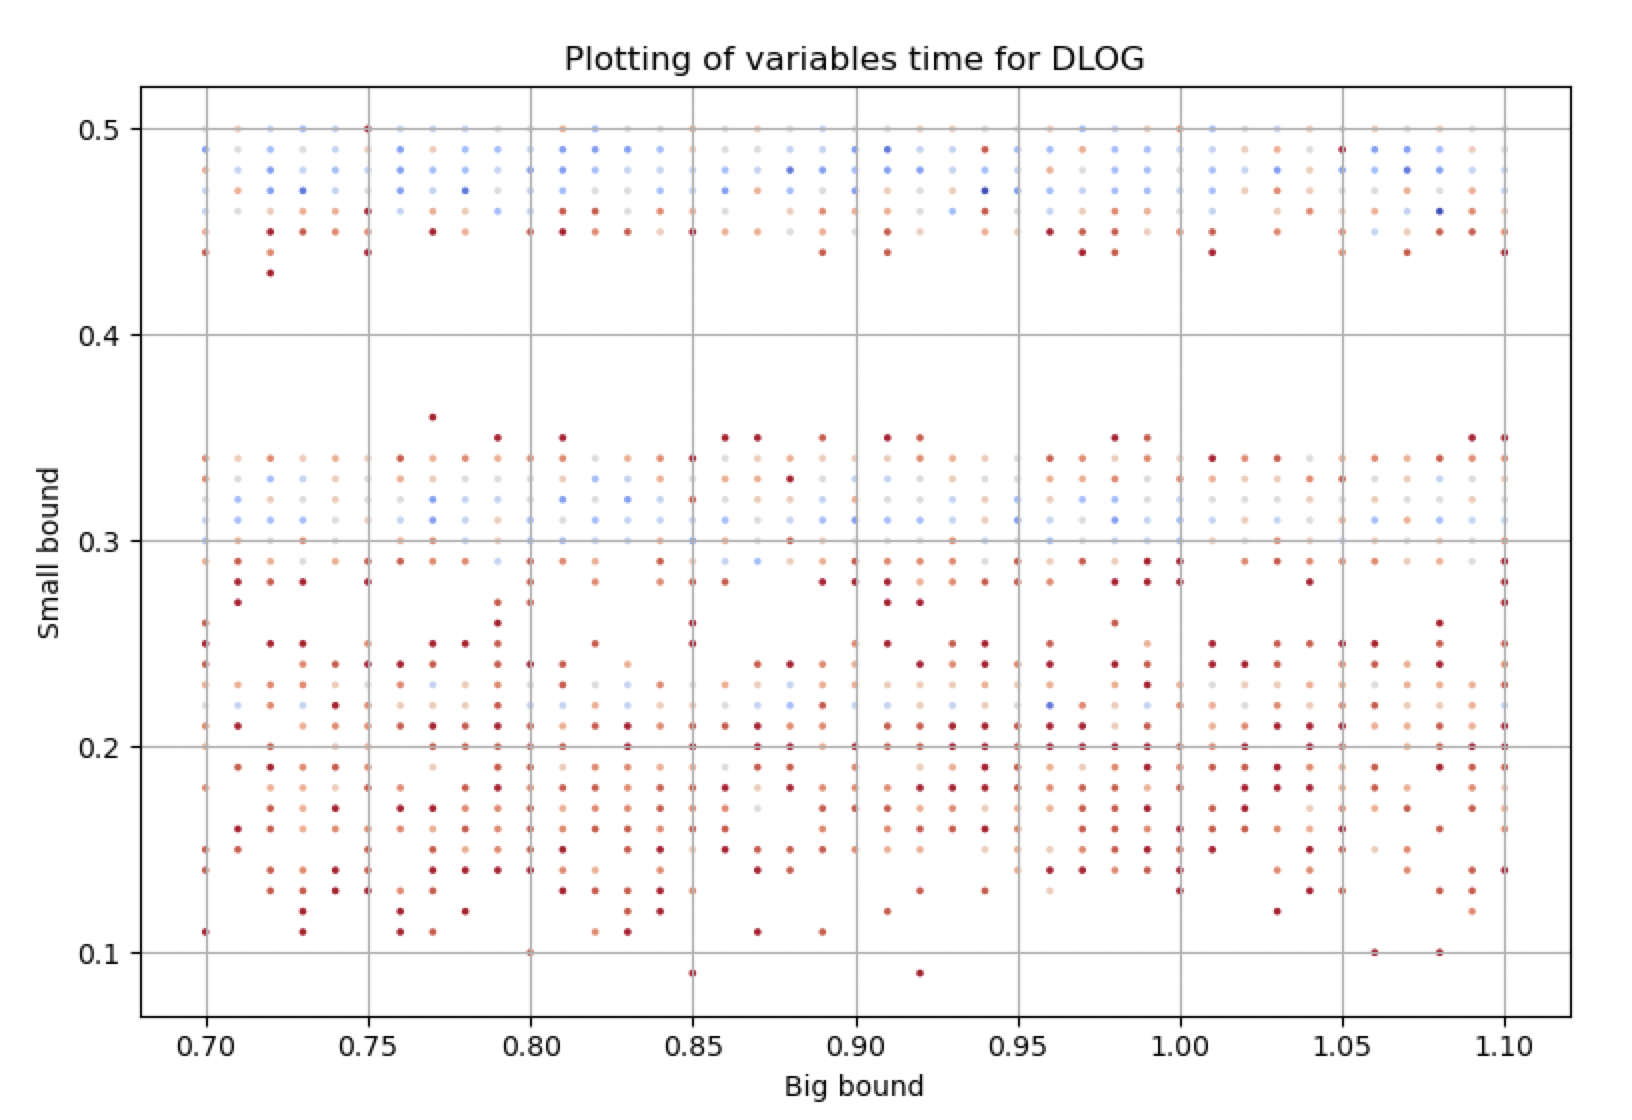
\includegraphics[width=\textwidth]{dlog_plot2d.png}
    \caption{Bounds in 2D, blue is faster.}
  \end{minipage}
  \hfill
  \begin{minipage}[b]{0.4\textwidth}
    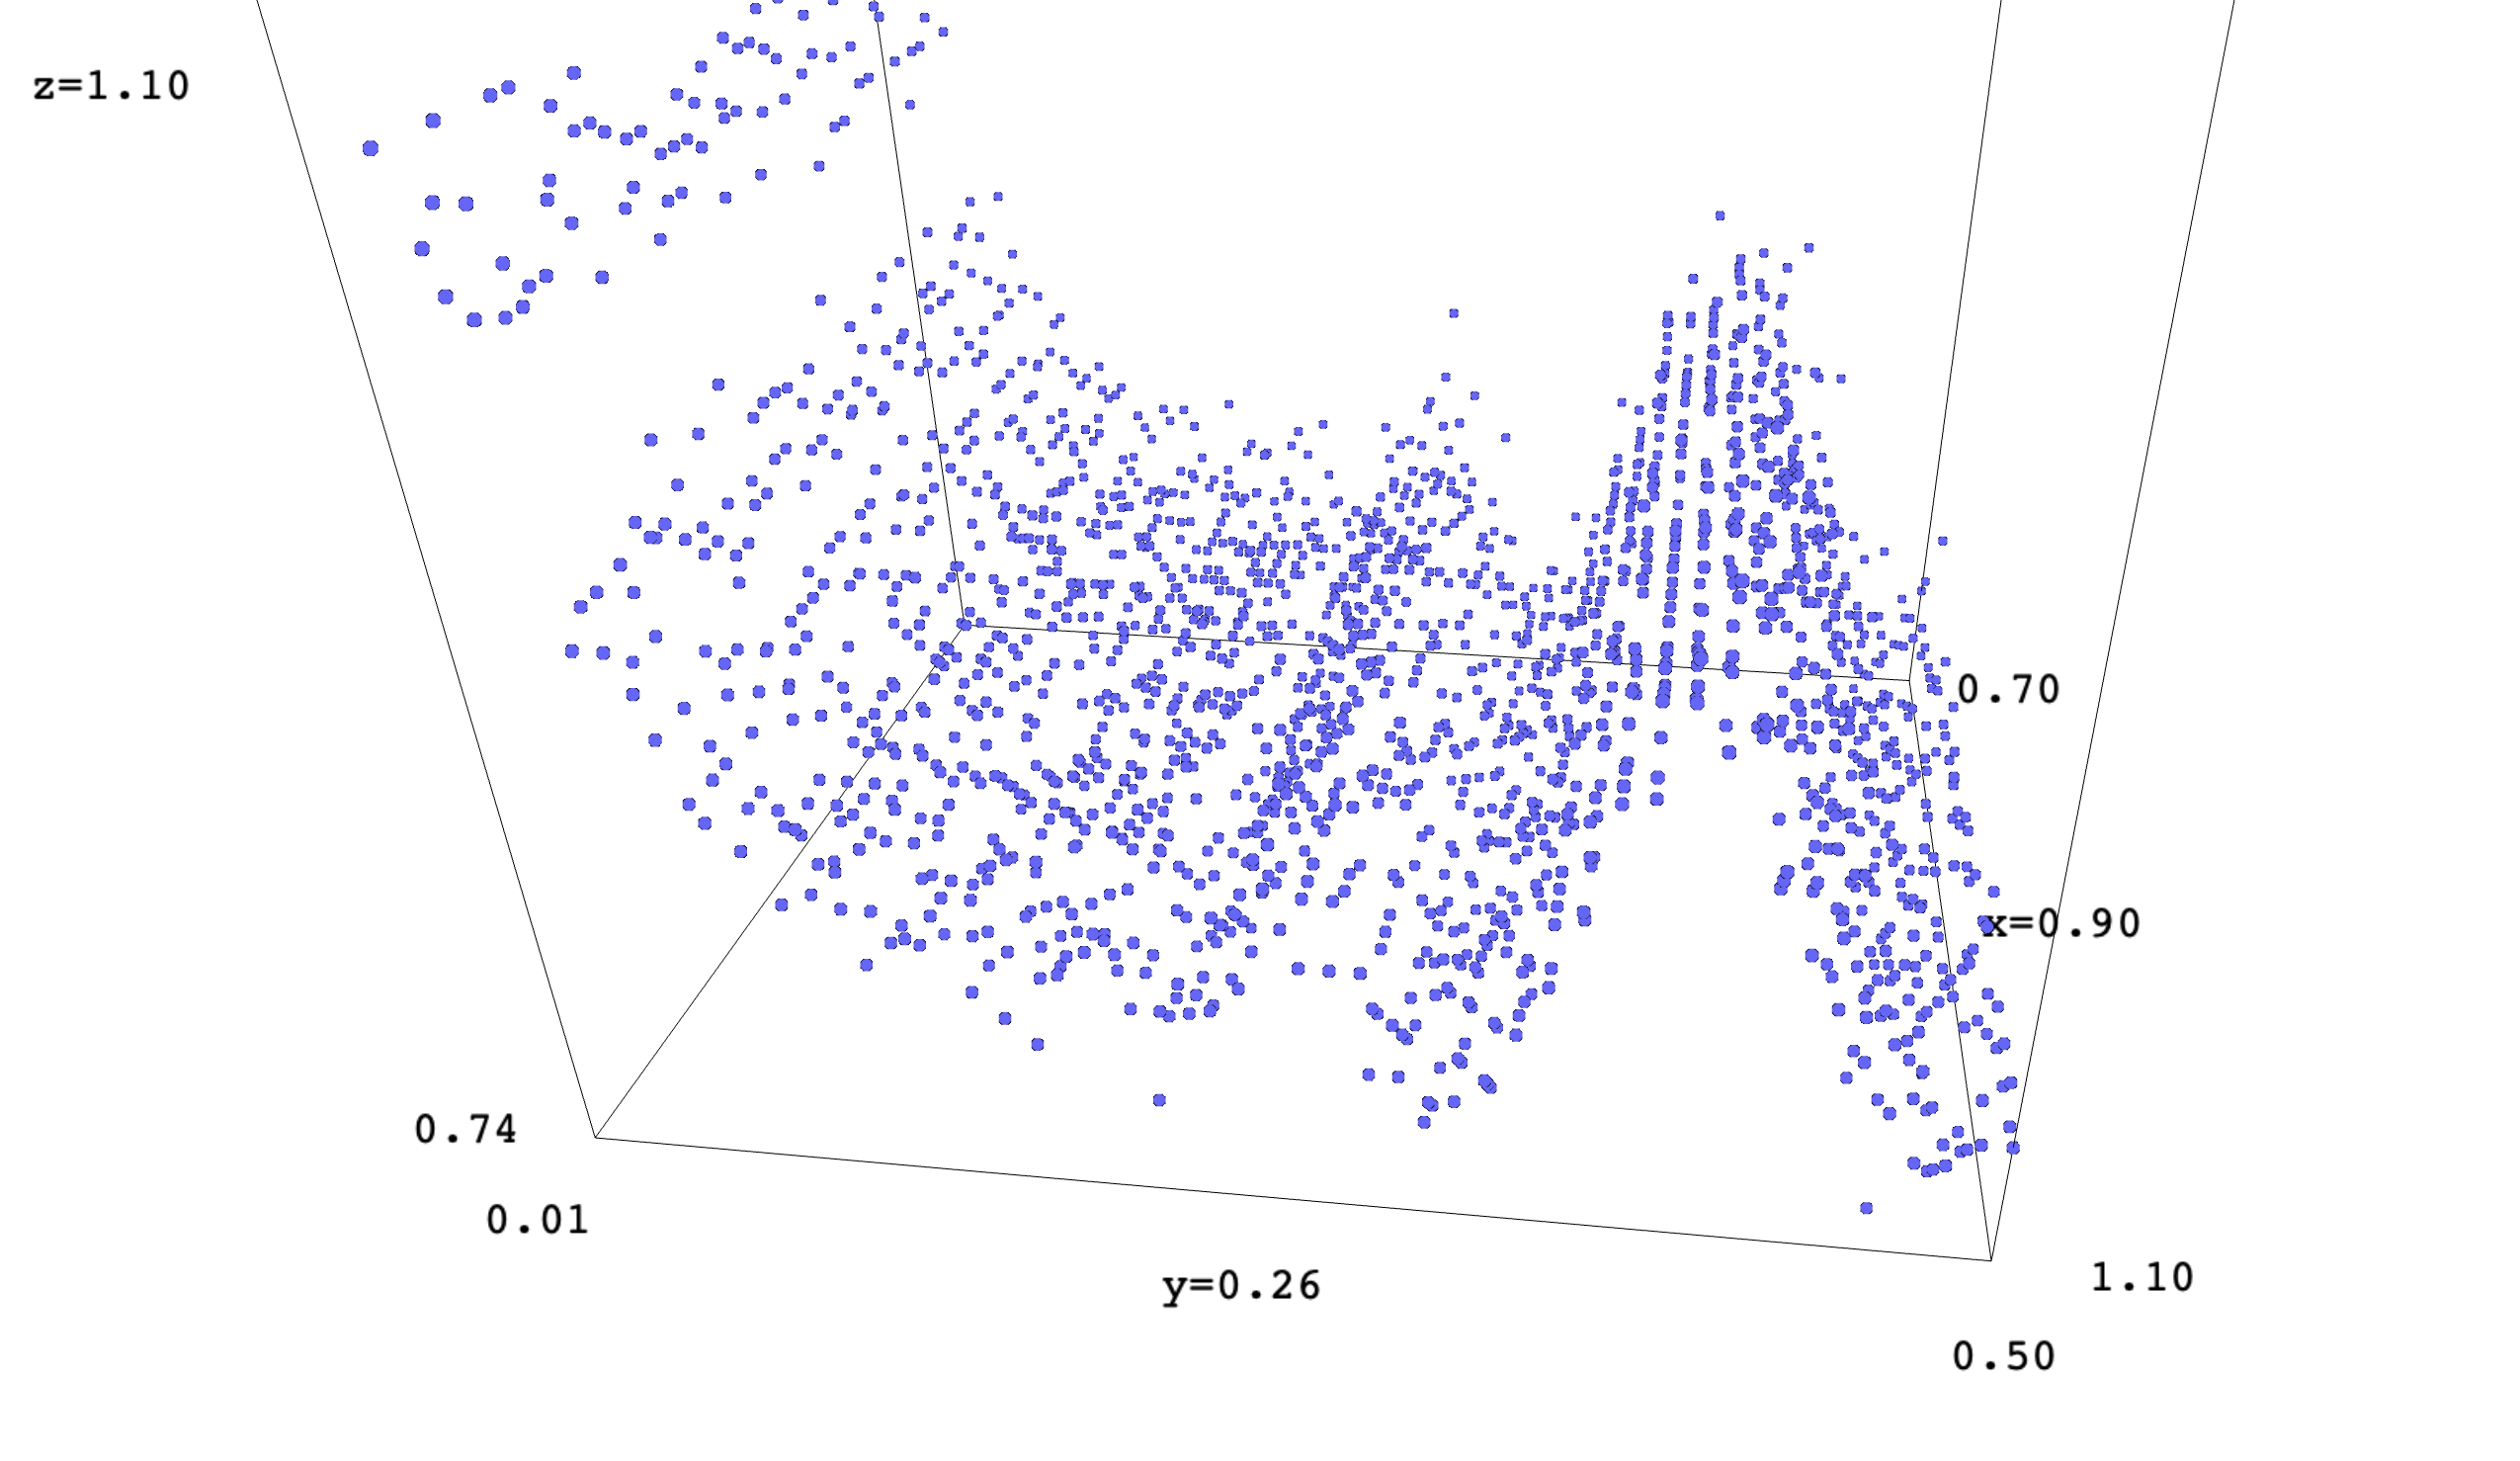
\includegraphics[width=\textwidth]{dlog_plot3d.png}
    \caption{Bounds in 3D.}
  \end{minipage}
\end{figure}





\subsubsection{The factor base}\label{sssec:fact_base}
Dario found the optimal bound




\section{Solovay-Strassen}

The Solovay-Strassen test is a primality test based on the Euler's criterion:
\begin{teo}\label{teo:eu_quad}
	If $p$ is a prime integer, than for any integer $a \in \ZZ$ we have:
	\[ a^{\frac{p-1}{2}} \equiv \left(\dfrac{a}{p}\right) \mod p \]
\end{teo}

The term on the right is the Legendre Symbol, that is equal to $0$ if $p$ divides $a$, to $1$ if it is a quadratic residue modulo $p$\footnote{if exists $b$ integer such that $a \equiv b^2 \mod p$} and $-1$ otherwhise. The generalization of the Legendre Symbol for all integers $n = p_1^{e_1} \cdots p_r^{e_r}$ is the Jacobi Symbol: 

\[ \left(\dfrac{a}{n}\right) := \left(\dfrac{a}{p_1}\right)^{e_1} \cdots \left(\dfrac{a}{p_r}\right)^{e_r} \] 
	
Since for general composite integers the theorem \ref{teo:eu_quad} won't always hold we can exploit this for a primality test. Given an odd integer $n$ the idea is to evaluate the two terms on a random integer $a\in \{2,...,n-1\}$ separately, see if they are equal, if no then $n$ is composite, otherwhise we change $a$ and repeat. We can conclude that $n$ is composite also if the Jacobi Symbol is equal to $0$, in fact this would imply that exists a prime $p_i$ dividing $a<n$ and $n$, so $n$ has a proper factor (in common with $a$). 

\begin{prob}\label{prob:jacobi}
	How do we evaluate the Jacobi Symbol without knowing the factorization of $n$?
\end{prob}

\begin{prob}\label{prob:eff_ss}
	What is the probability for a composite number to pass the test $m$ times?
\end{prob}

It is possible to prove that no composite number pass the test for all $a\in\{0,...,n-1\}$ and in particular it fails in at least $1/2$ of them. So we have that 
\begin{equation}
	\label{eq:prob_SS}
\PP(n \text{ pass the SS test }m\text{ times}|n\text{ is composite})\leq \frac{1}{2^m} .
\end{equation}
Observe that what we want is $\PP(n\text{ is composite}|n \text{ pass the SS test }m\text{ times})$, but it is possible to use Bayes' theorem to compute:
\begin{equation}
	\label{eq:prob_SS_good}
	\PP(n\text{ is composite}|n \text{ pass the SS test }m\text{ times})
	\leq
	\frac{\log(n) - 2}{\log(n) - 2 + 2^{m+1}}
\end{equation}

You can see the proof of this at page 208 of \cite[Section 6.4.2]{stinson}.

In our implementation we repeat the test $m=10$ times and the test vectors are integers $n \approx 2^20 \approx e^{13.9}$, se we get a pseudoprime with probability:
\begin{equation*}
	\leq frac{13.9 - 2}{13.9 - 2 + 2^{11}} \approx 0.00577
\end{equation*}

Is likely that the real probability is less, since I was unable to find a counter example.

So we have partially solved problem \ref{prob:eff_ss}, we focus now on problem \ref{prob:jacobi}. In the code I have solved this problem using the native MAGMA function \texttt{JacobiSymbol}, clearly very fast, but I want however to show a simple way to evaluate it (also implemented in the file, but not used) without the factorization to prove we can solve problem \ref{prob:jacobi}.

The idea is to use some of the properties of the Jacobi Symbol (inherited from the corresponding ones of the Legendre Symbol) to reduce the problem to it's evaluation on $0$, $1$ (trivial) and $2$. I insert the property in the order in which they are used. 
\begin{enumerate}
	\item We can evaluate $ \left(\dfrac{2}{n}\right) $ as $1$ for $n\equiv \pm 1 \mod 8$ and $-1$ otherwhise. Also we have $ \left(\dfrac{ac}{n}\right) = \left(\dfrac{a}{n}\right)  \left(\dfrac{c}{n}\right) $. So if $a = 2^km$ (with $m$ odd) we have that:
	\begin{itemize}
		\item $\left(\dfrac{a}{n}\right) = \left(\dfrac{m}{n}\right)$ for $k$ even or $n\equiv \pm 1 \mod 8$ 
		\item $\left(\dfrac{a}{n}\right) = -\left(\dfrac{m}{n}\right)$ otherwhise
	\end{itemize}
	\item $\left(\dfrac{a}{n}\right) = - \left(\dfrac{n}{a}\right)$ for $m \equiv n \equiv 3 \mod 4$ and $\left(\dfrac{m}{n}\right) = \left(\dfrac{n}{m}\right)$ otherwhise
	\item $\left(\dfrac{a}{n}\right) = \left(\dfrac{a \mod n}{n}\right)$
\end{enumerate}

We repeat these steps until $a\in\{0,1\}$ memorizing the sign changes. We then return the sign if $a=1$, and $0$ otherwhise.

Since the case in which we return $0$ is equivalent to $a$ having a common factor we can avoid calculation verifying in advance if $\gcd(a,n) \neq 1$, eventually returning $0$. 

\subsection{Final remark on the implementation}

There isn't much more to say with respect to the implementation, in fact the only two expensive part are the evalutations of the Jacobi Symbol (very efficient using the native function) and of $a^{\frac{n-1}{2}} \mod n$ (done with \texttt{Modexp}). All the other changes that I have tried, for example the way to check $x\equiv y \mod n$, didn't improve the time.  



\section{Lehman}

The Lehman factorization algorithm is a modification of the Fermat factorization algorithm proposed in \cite{lehman}. It has complexity of $O(n^{1/3})$ and it was the first hystorical example of an algorithm with time complexity less than $O(n^{1/2})$. 

The principal result of the article is the following theorem:

\begin{teo} \label{teo:lehm}
	Suppose that $n = pq$ is a positive odd integer, with $p,q$ primes, and consider and integer $r \in \{ 1,...,\lfloor n^{1/2}\rfloor\}$. Suppose that it holds:
	\begin{equation}
		\label{eq:p_cond}
		\left( \frac{n}{r+1}\right)^{1/2} < p \leq n^{1/2}
	\end{equation}
	Then there exists non negative integers $x,y$ and $k \in \{1,...,r\}$ such that:
	\begin{subequations} \label{eq:lehm_cond}
		\begin{align}
			&x^2 - y^2 = 4kn, \label{eq:lehm_cond_xy}\\
			&x \equiv k + 1 \mod 2, \label{eq:lehm_cond_1} \\
			&x \equiv k + n \mod 4 \text{ if k is odd},\label{eq:lehm_cond_2} \\
			&0 \leq x - (4kn)^{1/2} \leq \frac{1}{4(r+1)} \left(\frac{n}{k}\right)^{1/2} \label{eq:lehm_cond_it}
		\end{align}
	\end{subequations}
	and we can use $x,y$ to factor $n$:
	\begin{equation}
		\label{eq:lehm_fact}
		\{p,q\} = \{\gcd(x+y,n), \gcd(x-y,n)\}
	\end{equation}
	Instead if $n$ is prime no integers satisfy the equations in \ref{eq:lehm_cond}.
\end{teo}

So using the theorem we can write a factorization algorithm for semiprimes:
\begin{enumerate}
	\item \label{enum:trial_div} Do trial division up to $\left( \frac{n}{r+1}\right)^{1/2}$, since we can find only primes that satisfy equation \ref{eq:lehm_cond}.
	\item Iterate for $k \in \{ 1,...,r\}$ 
	\item \label{enum:lehm_xit} Iterate for $x \in \{ \lfloor (4kn)^{1/2}\rfloor , ..., \lceil \frac{1}{4(r+1)} \left(\frac{n}{k}\right)^{1/2} + (4kn)^{1/2} \rceil \}$ such that $x \equiv k + 1 \mod 2$ and, if $k$ is odd, $x \equiv k + n \mod 4$
	\item If $x^2 - 4kn$ is a perfect square $y^2$ return the factorization: 
		$$\{\gcd(x+y,n), \gcd(x-y,n)\}$$
	\item If we can't find any factor after all the iterations we return that $n$ is prime.
\end{enumerate}

The trial division require $O\left( \left( \frac{n}{r}\right)^{1/2} \right)$ operations, while for each $k$ we have $O\left( \frac{1}{r} \left(\frac{n}{k}\right)^{1/2} \right)$ possible $x$ to check (there is also a constant quantity of operations to perform in order to evaluate the interval). So the total operations are:
\begin{equation}
	\label{eq:lehm_compl}
	O\left( \left( \frac{n}{r}\right)^{1/2} \right) + \sum_{k =1}^r O\left( \frac{1}{r} \left(\frac{n}{k}\right)^{1/2} + 1\right)
\end{equation}

that for $r = O(n^{1/3})$ can be approximated to a complexity of $O(n^{1/3})$. This choice is not proven to be optimal, in fact for the calculation it is used that $ \sum_{i=1}^r O\left( \frac{1}{k^{1/2}}\right) \subset O(r^{1/2})$, and I think that we can do better (at least emprically I have observed that for $r = n^(1/4)$ we can do better).

\subsection{Implementation}

In \cite[Section 5]{lehman} is also inserted the algorithm written in \texttt{Algol} with some ideas to improve velocity, that I have followed in the MAGMA implementation. 

First we define the function \texttt{isqrt} that returns $\lceil n^{1/2}\rceil$ and $\lceil n^{1/2}\rceil^2 - n$. It uses both \texttt{Sqrt} and \texttt{Ceiling}. 

Then we initialize a boolean array \texttt{QR} (outside of the function), the value of $r$ as $\lceil n^{1/4} \rceil$ and a sequence of arrays \texttt{C}. 

%\begin{wrapfigure}{r}{0.5\textwidth}
% \begin{center}
%   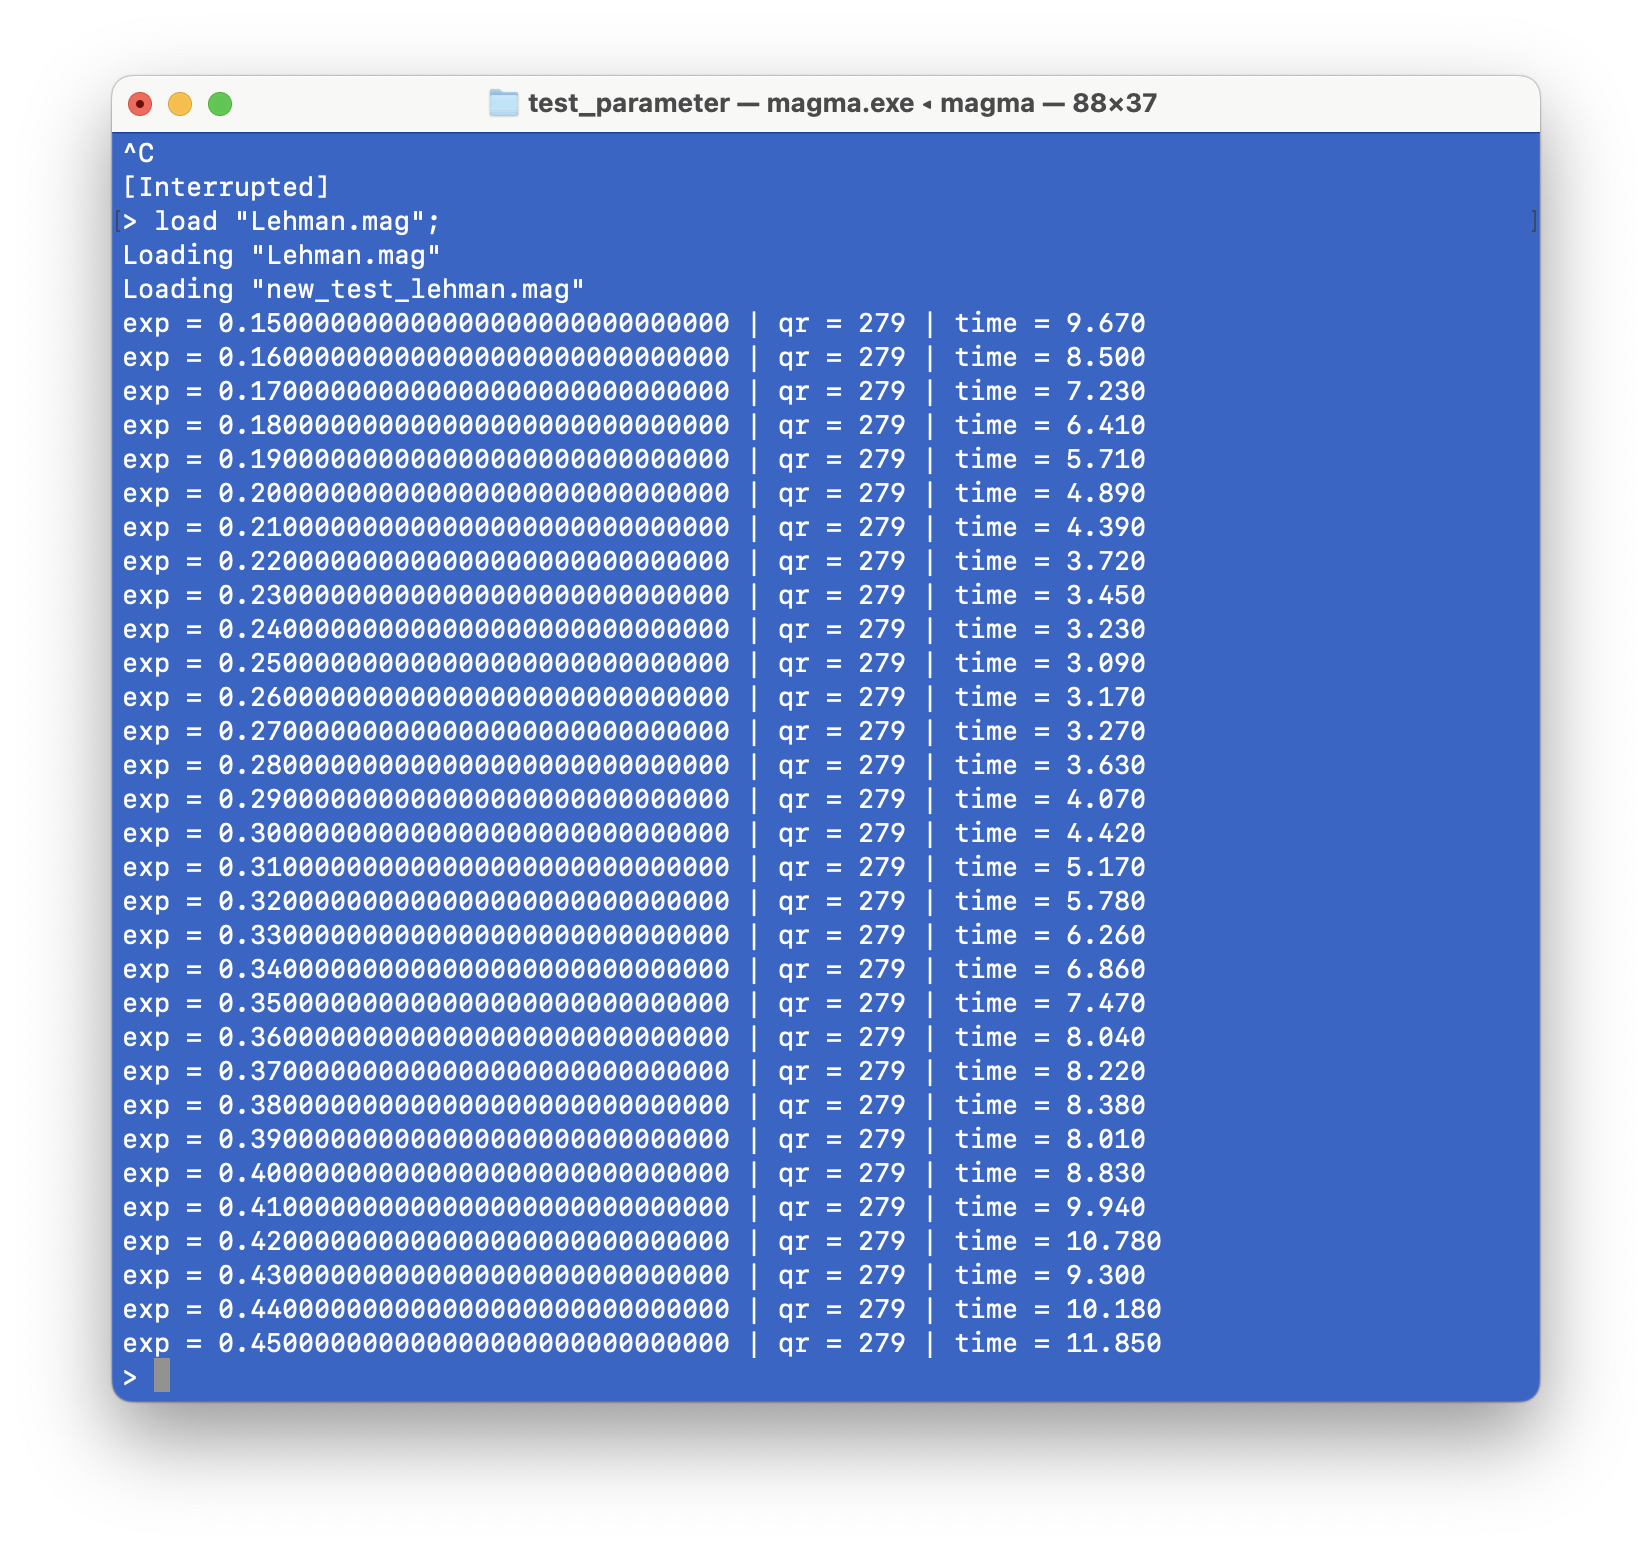
\includegraphics[width=0.45\textwidth]{r_coiche.png}
% \end{center}
%   \label{fig:r_choice}
%  \caption{Time for $r = n^{exp }$ }
%\end{wrapfigure}


\begin{figure}[!tbp]
  \centering
  \begin{minipage}[b]{0.5\textwidth}
	\label{fig:r_choice}
    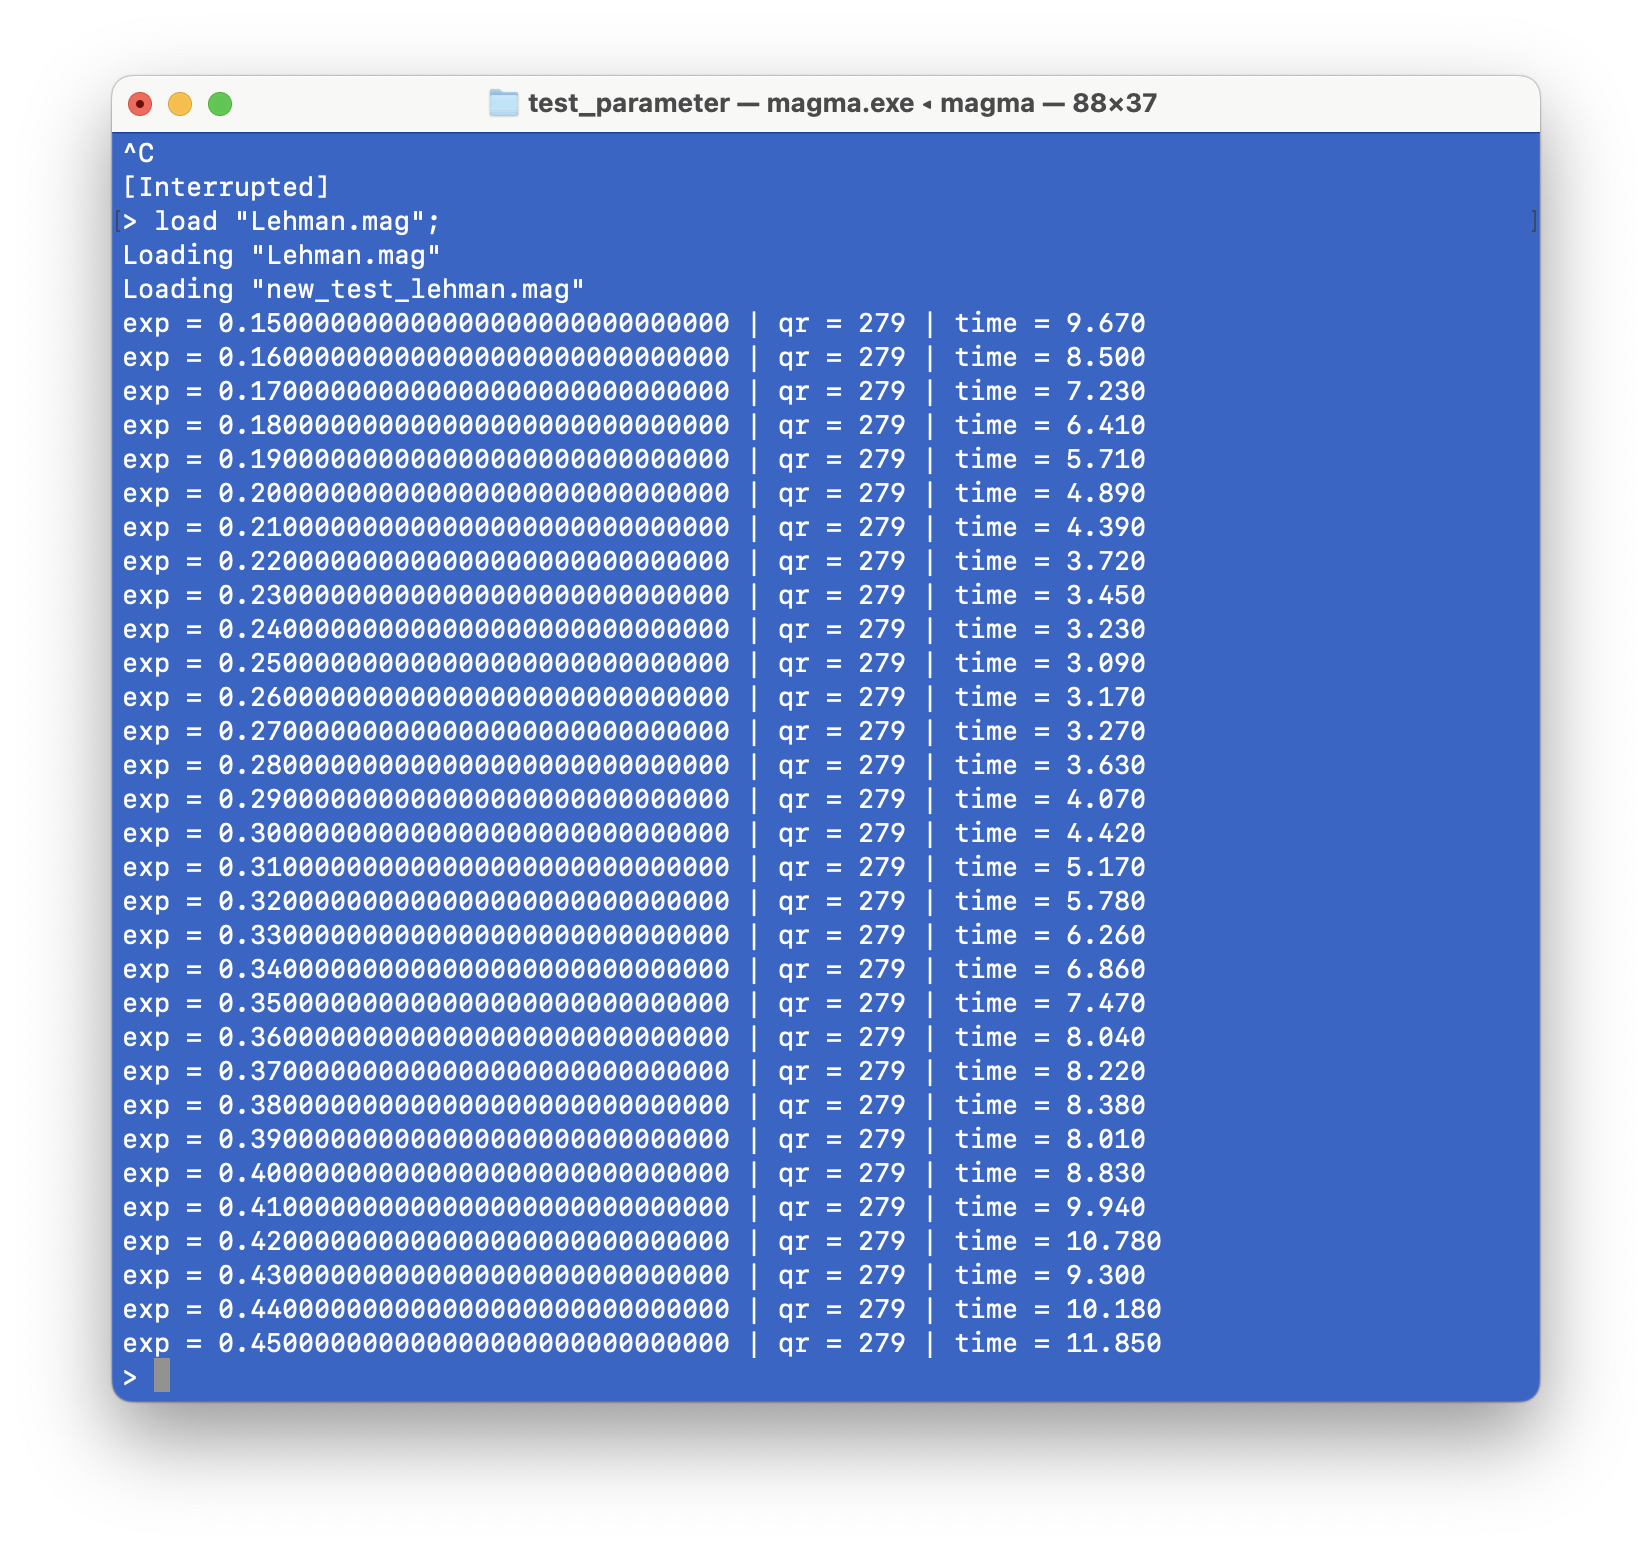
\includegraphics[width=\textwidth]{r_coiche.png}
    \caption{Time for $r = n^{exp }$ }
  \end{minipage}
  \hfill
  \begin{minipage}[b]{0.45\textwidth}
	  \label{fig:qr_choice}
    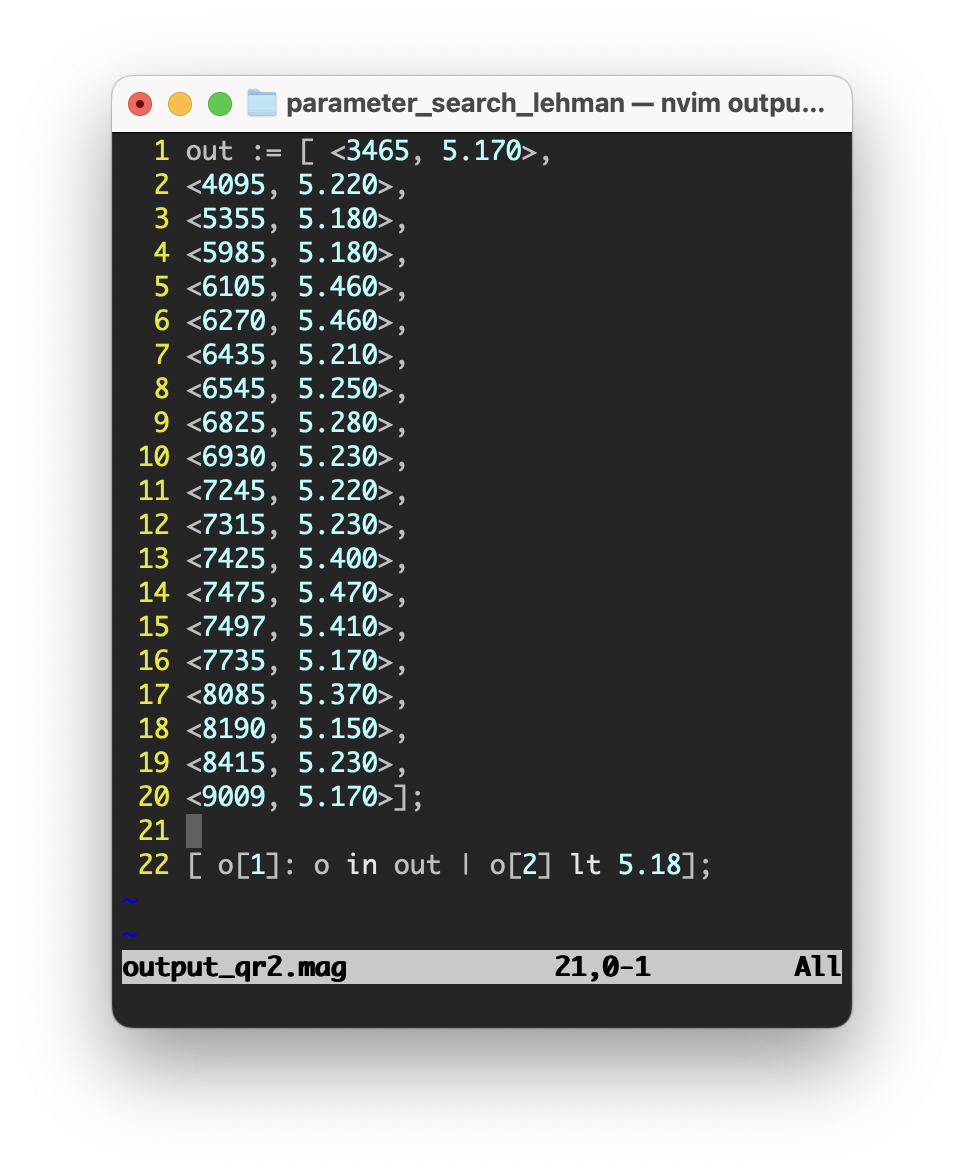
\includegraphics[width=\textwidth]{qr_choiche.png}
    \caption{optimal qr mod with factorization and time}
  \end{minipage}
\end{figure}


\begin{rem}
	Statistical tests showed that $r = n^{1/4}$ achieves better performances, as it can be seen in Figure \ref{fig:r_choice}. I have tried them because I wasn't conviced by the big $O$ calculations in the article and, at least emprically, I can claim $n^{1/4}$ to be better. 

	Observe that in our case we have $p \approx q \approx 2^{20}$, so $n\approx 2^{40}$ and $r = n^{1/4} \approx 2^{10}$. For the theorem \ref{teo:lehm} we need equation \ref{eq:lehm_cond} to be satisfied, i.e.:
	\begin{equation*}
		\left(\frac{n}{r+1}\right)^{1/2} \approx \left( 2^{40-10} \right)^{1/2} \approx 2^{15} << 2^{20} \approx p
	\end{equation*} 
\end{rem}

In the article the authors observed that $k$ with an higher number of divisors are more likely to find a factorization, thus we should try them first. 
The arrays in \texttt{C} are necessary to iterate over $k \in \{1,...,r\}$ passing before from numbers with more divisors, for example the multiple of $30$ and of $24$. Each \verb|array| contains a starting value for $k$ \verb|array[2]| that it is incremented using the elements of \verb|array[3]| cycled modulo \verb|array[1]| (the lenght of \verb|array[3]|). When $k > r$ then we change array. Observe that the odd $k$ values are done last (we will use this later). 

Then we define $x := \lceil (4kn)^{1/2}\rceil $ and $ u := x^2 - 4kn$ (it is the candidate to $y^2$ as in \ref{eq:lehm_cond_xy}). The next two \texttt{if} conditions increment $x$ to have the conditions \ref{eq:lehm_cond_1} and \ref{eq:lehm_cond_2}. Observe that also $u$ is incremented using that:
\begin{equation}
	\label{eq:incr_u}
	(x+b)^2 - 4kn = \underbrace{(x^2 - 4kn)}_{\text{previous }u} + 2\cdot b \cdot x + b^2
\end{equation}
So we don't have to evaluate other square roots. 

When we have the first $x$ we can start the iteration, incrementing by $\verb|jump| = 2$ for $k$ even and $4$ othewhise, using again the tecnique in equation \ref{eq:incr_u}. By the condition \ref{eq:lehm_cond_it} we have to iterate over \verb|[i1..(j+1) by jump]| where \verb|i1| is the number of $x$ skipped previously. 

The only thing we miss now is to check whether or not $u$ is a perfect square $y^2$. Here we will use the boolean array \texttt{Qr}, 
that it was initliazed by performing square modulo \verb|qr_mod| and setting to \texttt{true} only the quadratic residues. 
The idea is to use that if $u$ is a perfect square, then it is a quadratic residue modulo \verb|qr_mod|. 
So if \verb|Qr[u mod qr_mod]| is \texttt{false} surely it is not a perfect square. 
Since in MAGMA the arrays start from $1$ we need to sligtly modify the modulo using some $-1$ and $+1$. 

In the article \verb|qr_mod|$=729=3^6$ is used because the percentage of quadratic residues is approximately $ 38 \%$, but I have observed that we can do better. For example $385 = 5 \cdot 7 \cdot 11$ has only $18.7 \%$ of quadratic residues and gives more efficient results during computations.  
I have actually tried all the possible \verb|qr_mod| up to $10000$, finding better choices (inserted in the code), and I have individuated as more efficient the value $3465 = 3^2 \cdot 5 \cdot 7 \cdot 11$. There where other possible good values, as you can see in figure \ref{fig:qr_choice}, all odd (but one) and with small factors. 
They have all small factors because this reduce the quantity of quadratic residues (remind that for the Chinese reminder theorem an integer is a quadratic residue for $n$ if it is a quadratic residue modulo all the factors $p^e$ of $n$).

I think that they are odd because we start the iteration on the even $k$, so $x \equiv k+1 \equiv 1 \mod 2$ is odd, thus $u = x^2 - 4kn$ is odd, hence the distribution of the non quadratic residue is able to spot more non-squares. 

\newpage
\printbibliography


\end{document}
